%%%%%%%%%%%%%%%%%%%%%%%%%
% Imports and Setup     %
%%%%%%%%%%%%%%%%%%%%%%%%%

\input{../lib/hw-setup/tex/HWSetup}
\input{../lib/hw-setup/tex/EngBindings}
\usetikzlibrary{arrows.meta, decorations.markings, patterns, calc, positioning}

\fancyhead[C]{}
\fancyhead[R]{\hyperlink{tableofcontents}{\hmwkClass\ (\hmwkClassInstructor,\ \hmwkClassTime): \hmwkTitle}}
\fancyheadwidth[L]{0.5\headwidth}
\fancyheadwidth[C]{0.0\headwidth}
\fancyheadwidth[R]{0.5\headwidth}

%%%%%%%%%%%%%%%%%%%%%%%%%
% Homework Details      %
% - Title               %
% - Subtitle            %
% - Due Date            %
% - Due Time            %
% - Course              %
% - Section Time        %
% - Instructor          %
% - Author              %
% - Submission Time     %
%%%%%%%%%%%%%%%%%%%%%%%%%

\hwkTitle{Lab01}
\hwkSubTitle{Pressure Measurements of Inviscid Flow over Cylinder}
\hwkDueDate{2026-02-13}
\hwkDueTime{11:59:00}
\hwkClass{ENAE464 - 0202}
\hwkClassTime{14:00:00}
\hwkInstructor{Dr. Silbaugh}
\hwkAuthor{Mikołaj Kostrzewa \& Vai Srivastava}
\hwkCompletionDate{
        Experiment Performed: \DTMdate{2026-02-06}\\
        Report Submitted: \DTMtoday
}

\addbibresource{./references.bib}

\begin{document}

\hypertarget{titlepage}{\maketitle}
\thispagestyle{empty}

\pagebreak

%%%%%%%%%%%%%%%%%%%%%%%%%
% Letter of Transmittal %
%%%%%%%%%%%%%%%%%%%%%%%%%

\thispagestyle{empty}

\DTMtoday

\vspace{5.0ex}

Enclosed is the technical report for the Flow Over Cylinder laboratory experiment. This report presents the experimental methodology, results, and analysis of flow characteristics observed around a circular cylinder, including pressure distribution, drag coefficient determination, and comparison with theoretical predictions.

Please feel free to contact us with any questions regarding the contents of this report.

\vspace{5.0ex}

Respectfully,

Mikołaj Kostrzewa \& Vai Srivastava

%%%%%%%%%%%%%%%%%%%%%%%%%
% Table of Contents     %
%%%%%%%%%%%%%%%%%%%%%%%%%

\pagebreak

\thispagestyle{empty}
\hypertarget{tableofcontents}{\tableofcontents}

\renewcommand{\listfigurename}{Figures}
\listoffigures

\renewcommand{\listtablename}{Tables}
\listoftables

\renewcommand{\listlistingname}{Listings}
\listoflistings

\newpage
\pagenumbering{arabic}

%%%%%%%%%%%%%%%%%%%%%%%%%
% Report                %
%%%%%%%%%%%%%%%%%%%%%%%%%

\section{Abstract} \label{sec:abstract}

This report presents the results of an experimental investigation of the pressure distribution over a circular cylinder of diameter \qty{1.27}{\cm} in a vertical wind tunnel. Surface pressure measurements were obtained by rotating a single pressure tap in \qty{5}{\deg} increments from \qty{0}{\deg} to \qty{180}{\deg}, and the freestream velocity was determined from pitot-static tube readings via Bernoulli's equation. The measured pressure coefficient distribution was compared with the inviscid potential flow prediction \(C_p=1-4 \oldsin ^2 \theta\), and the drag coefficient was computed by trapezoidal integration of the surface pressure. The experimental data agreed closely with inviscid theory over the forward portion of the cylinder \(\left(\qty{0}{\deg} \leq \theta \leq \qty{30}{\deg}\right)\), but diverged significantly beyond \(\theta \approx \qty{30}{\deg}\), where boundary layer separation caused the pressure coefficient to plateau near \(C_p \approx-1\) rather than reaching the theoretical minimum of \(-3\). The resulting asymmetry between fore and aft pressure yielded a nonzero drag coefficient, in contrast to the zero-drag prediction of inviscid theory (d'Alembert's paradox).

\section{Introduction} \label{sec:introduction}

For the inviscid-flow model used in this lab, we assume a potential-flow field that is:
\begin{itemize}
    \item \textbf{Incompressible (continuity):} \(\nabla \cdot \vec{V} = 0\).
    \item \textbf{Irrotational:} \(\nabla \times \vec{V} = 0\).
\end{itemize}
If \(\nabla \times \vec{V} = 0\), then a \textit{velocity potential} \(\phi\) exists such that
\(\vec{V}=\nabla \phi\). Substituting into continuity gives Laplace's equation:
\begin{equation}
    \nabla^2 \phi = 0
    \qquad \left(\text{i.e., } \frac{\partial^2 \phi}{\partial x^2}
    + \frac{\partial^2 \phi}{\partial y^2}
    + \frac{\partial^2 \phi}{\partial z^2} = 0 \right).
\end{equation}

In order to model flow over a 2D cylinder, we use an approach presented in \cite{danderson2023fundamentals}, which uses a superposition of a uniform flow and a doublet flow, as presented in the figure below \cite[Fig.~3.26]{danderson2023fundamentals}:

\begin{figure}[H]
    \centering
    \includegraphics[width=0.65\linewidth]{../assets/flow_superposition.png}
    \caption{Superposition of uniform flow and a doublet to model nonlifting potential flow over a circular cylinder.}
    \label{fig:flow_superposition}
\end{figure}

In polar coordinates \((r,\theta)\), the stream function and velocity potential for both the uniform flow and the doublet are given by:
\begin{align}
    \phi_U &= V_{\infty} r \cos\theta
    && \text{(velocity potential: uniform flow)} \\
    \psi_U &= V_{\infty} r \sin\theta
    && \text{(stream function: uniform flow)} \\
    \phi_D &= \frac{\kappa}{2\pi}\frac{\cos\theta}{r}
    && \text{(velocity potential: doublet)} \\
    \psi_D &= -\frac{\kappa}{2\pi}\frac{\sin\theta}{r}
    && \text{(stream function: doublet)}
\end{align}
where \(V_{\infty}\) is the freestream speed and \(\kappa\) is the doublet strength.

Superposing the uniform flow and doublet stream functions gives
\begin{align}
    \psi &= \psi_U + \psi_D \\
    &= V_{\infty} r \sin\theta - \frac{\kappa}{2\pi}\frac{\sin\theta}{r} \\
    &= V_{\infty} r \sin\theta \left(1 - \frac{R^2}{r^2}\right),
\end{align}
where the cylinder radius is defined by
\begin{equation}
    R^2 \equiv \frac{\kappa}{2\pi V_{\infty}}.
\end{equation}

The corresponding velocity field in polar coordinates follows from the stream function relations
\(V_r=\frac{1}{r}\frac{\partial \psi}{\partial \theta}\) and \(V_{\theta}=-\frac{\partial \psi}{\partial r}\):
\begin{align}
    V_r &= \frac{1}{r}\frac{\partial \psi}{\partial \theta} = \frac{1}{r}\left(V_{\infty} r \cos\theta\right)\left(1-\frac{R^2}{r^2}\right) \\
        &= \left(1-\frac{R^2}{r^2}\right)V_{\infty}\cos\theta, \\
    V_{\theta} &= -\frac{\partial \psi}{\partial r} \\
               &= -\left(1+\frac{R^2}{r^2}\right)V_{\infty}\sin\theta.
\end{align}

At the surface of the cylinder, \(r = R\), the velocity field is:
\begin{align}
    V_r &= \left(1-\frac{R^2}{R^2}\right)V_{\infty}\cos\theta = 0, \\
    V_{\theta} &= -\left(1+\frac{R^2}{R^2}\right)V_{\infty}\sin\theta = -2V_{\infty}\sin\theta.
\end{align}

This aligns with the assumption that the velocity normal to the stationary surface must be zero, and due to polar coordinates, the velocity normal to the surface is given by \(V_{r}\).
Since \(V_{\theta}\) is perpendicular to the surface, due to construction of the coordinate system, it's equivalent to a tangential velocity, and since normal velocity is zero, \(V = V_{\theta} = V_{\infty} \sin\theta\).

The pressure coefficient is given by:
\begin{align}
    C_p &= 1 - \frac{V^2}{V_{\infty}^2} \\
    V &= -2V_{\infty}\sin\theta \\
    \frac{V^2}{V_{\infty}^2} &= 4\oldsin^2\theta
\end{align}
\begin{equation}
    \boxed{C_p = 1 - \frac{V^2}{V_{\infty}^2} = 1 - 4\oldsin^2\theta} \label{eq:introduction/Cp}
\end{equation}

\section{Experimental Apparatus and Procedures} \label{sec:procedures}

\subsection{Experimental Apparatus} \label{sec:procedures/apparatus}

The experimental apparatus for this lab consisted of a wind tunnel whose test chamber contained a small metal cylinder, with diameter \qty{1.27}{\cm}. This wind tunnel was oriented such that the flow of air through the test chamber happened from top to bottom. Being above the direction of flow, the air reservoir was set up to hold unpressurized air (being left only at ambient room pressure). From there, the air is accelerated through the test chamber, and exits out the back into the room. Installed in the test chamber is the cylinder, connected to a scale with demarcations at every \qty{5}{\deg}. Installed within the wind tunnel were 3 pitot-static tubes connected to a manometer: tracking the pressure in the reservoir \( P_{0} \), upstream of the cylinder \( P_{\infty} \), and on the surface of the cylinder \( P \)---aligned with the \qty{0}{\deg} angle.

\begin{figure}[H]
    \centering
    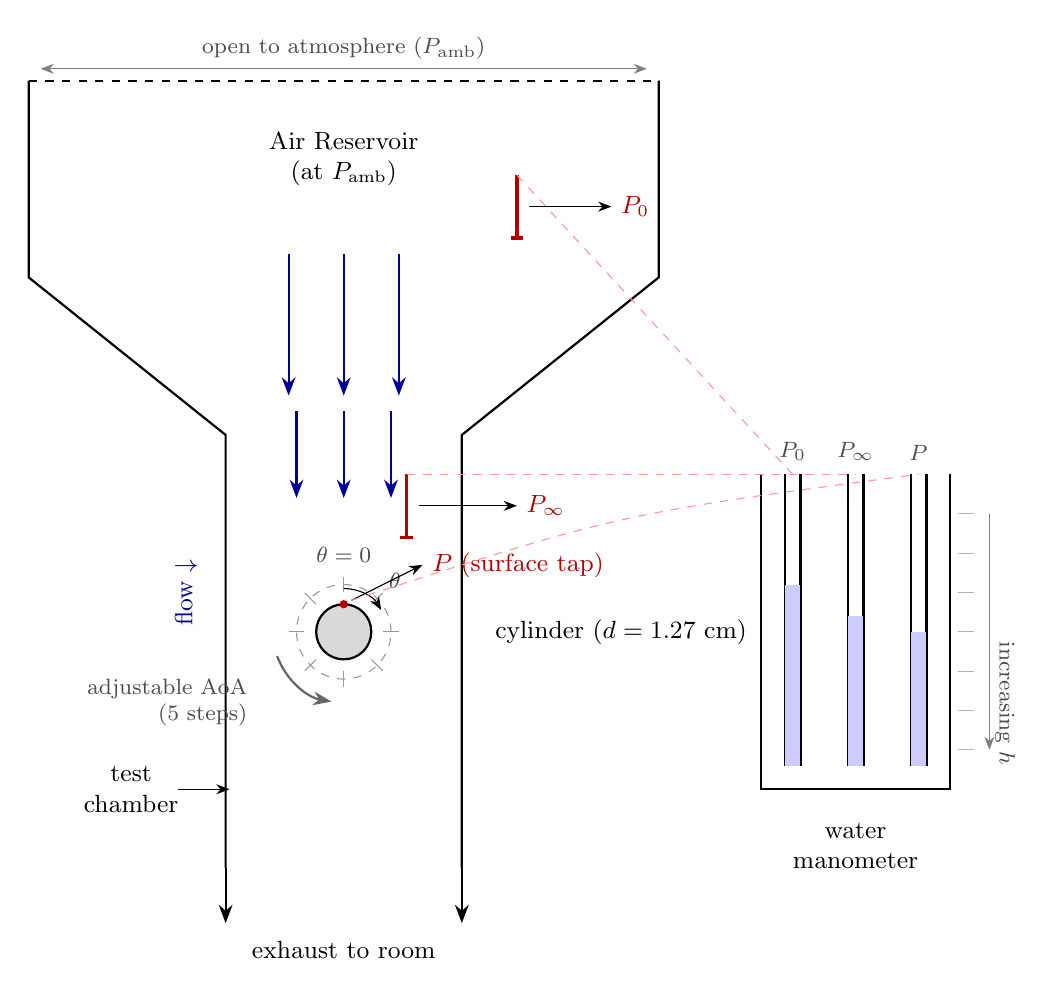
\begin{tikzpicture}[
            >=Stealth,
            flow arrow/.style={->, thick, blue!60!black},
            label text/.style={font=\small},
            dim text/.style={font=\footnotesize, text=black!70},
            pitot/.style={very thick, red!70!black},
        ]
        % ── Wind tunnel outline (vertical, flow top-to-bottom) ───────────────────────
        % Reservoir (top, wide)
        \def\resW{4}    % reservoir half-width
        \def\resH{2.5}  % reservoir height
        \def\resTop{10} % top of reservoir

        % Contraction
        \def\conH{2}    % contraction height
        \def\chW{1.5}   % test chamber half-width

        % Test chamber
        \def\chH{5}     % test chamber height
        \def\chBot{0}   % bottom of test chamber

        % Reservoir walls
        \draw[thick] (-\resW, \resTop) -- (-\resW, \resTop - \resH)
            -- (-\chW, \resTop - \resH - \conH)
            -- (-\chW, \chBot);
        \draw[thick] (\resW, \resTop) -- (\resW, \resTop - \resH)
            -- (\chW, \resTop - \resH - \conH)
            -- (\chW, \chBot);

        % Reservoir top (open to atmosphere)
        \draw[thick, dashed] (-\resW, \resTop) -- (\resW, \resTop);

        % "Open to atmosphere" label
        \draw[<->, thin, black!50] (-\resW+0.15, \resTop+0.15) -- (\resW-0.15, \resTop+0.15);
        \node[above, dim text] at (0, \resTop+0.15) {open to atmosphere ($P_{\mathrm{amb}}$)};

        % Reservoir label
        \node[label text, align=center] at (0, \resTop - 1.0) {Air Reservoir \\ (at $P_{\mathrm{amb}}$)};

        % Test chamber exit
        \draw[thick, ->] (-\chW, \chBot) -- (-\chW, \chBot - 0.7);
        \draw[thick, ->] (\chW, \chBot)  -- (\chW, \chBot - 0.7);
        \node[below, label text] at (0, \chBot - 0.8) {exhaust to room};

        % ── Flow arrows ──────────────────────────────────────────────────────────────
        \foreach \x in {-0.7, 0, 0.7} {
            \draw[flow arrow] (\x, \resTop - \resH + 0.3) -- (\x, \resTop - \resH - \conH + 0.5);
        }
        \foreach \x in {-0.6, 0, 0.6} {
            \draw[flow arrow] (\x, \resTop - \resH - \conH + 0.3) -- (\x, \resTop - \resH - \conH - 0.8);
        }
        % Flow label
        \node[label text, blue!60!black, rotate=90] at (-\chW - 0.5, 3.5) {flow $\downarrow$};

        % ── Cylinder ─────────────────────────────────────────────────────────────────
        \def\cylY{3.0}    % vertical position of cylinder centre
        \def\cylR{0.35}   % drawn radius (not to scale)

        \draw[fill=gray!30, thick] (0, \cylY) circle (\cylR);
        \node[label text, right] at (\chW + 0.3, \cylY) {cylinder ($d = 1.27$ cm)};

        % Angle scale ring (dashed)
        \draw[dashed, thin, black!40] (0, \cylY) circle (\cylR + 0.25);

        % Angle tick marks and labels (every 45° for clarity)
        \foreach \a/\lbl in {0/0, 45/45, 90/90, 135/135, 180/180, 225/225, 270/270, 315/315} {
            \draw[thin, black!40] ({\cylR + 0.15)*cos(\a)}, {\cylY + (\cylR + 0.15)*sin(\a)})
                -- ({(\cylR + 0.35)*cos(\a)}, {\cylY + (\cylR + 0.35)*sin(\a)});
        }

        % θ = 0° label (pointing upstream, i.e. upward towards flow)
        \node[above, dim text] at (0, \cylY + \cylR + 0.4) {$\theta = 0°$};

        % Angle arc
        \draw[->, thin] ({0.55*cos(90)}, {\cylY + 0.55*sin(90)}) arc[start angle=90, end angle=30, radius=0.55];
        \node[dim text] at (0.65, \cylY + 0.65) {$\theta$};

        % Adjustable rotation arrow
        \draw[->, thick, black!60] ({0.9*cos(200)}, {\cylY + 0.9*sin(200)})
            arc[start angle=200, end angle=260, radius=0.9];
        \node[left, dim text, align=right] at (-1.1, \cylY - 0.9) {adjustable AoA\\($5°$ steps)};

        % ── Pitot-static tube: P_0 (in reservoir) ───────────────────────────────────
        \def\ptX{2.2}
        \def\ptTopY{\resTop - 1.2}

        % Tube body
        \draw[pitot] (\ptX, \ptTopY) -- (\ptX, \ptTopY - 0.8);
        \draw[pitot] (\ptX - 0.08, \ptTopY - 0.8) -- (\ptX + 0.08, \ptTopY - 0.8); % tip
        % label
        \draw[thin, ->] (\ptX + 0.15, \ptTopY - 0.4) -- (\ptX + 1.2, \ptTopY - 0.4);
        \node[right, label text, red!70!black] at (\ptX + 1.2, \ptTopY - 0.4) {$P_0$};

        % ── Pitot-static tube: P_∞ (upstream of cylinder) ───────────────────────────
        \def\pinfY{5.0}

        \draw[pitot] (\ptX - 1.4, \pinfY) -- (\ptX - 1.4, \pinfY - 0.8);
        \draw[pitot] (\ptX - 1.48, \pinfY - 0.8) -- (\ptX - 1.32, \pinfY - 0.8);
        % label
        \draw[thin, ->] (\ptX - 1.25, \pinfY - 0.4) -- (\ptX + 0.0, \pinfY - 0.4);
        \node[right, label text, red!70!black] at (\ptX + 0.0, \pinfY - 0.4) {$P_\infty$};

        % ── Pressure tap on cylinder surface: P ──────────────────────────────────────
        % Small dot at θ = 0 (top of cylinder, facing flow)
        \fill[red!70!black] (0, \cylY + \cylR) circle (1.5pt);
        % line to label
        \draw[thin, ->] (0.1, \cylY + \cylR + 0.05) -- (1.0, \cylY + \cylR + 0.5);
        \node[right, label text, red!70!black] at (1.0, \cylY + \cylR + 0.5) {$P$ (surface tap)};

        % ── Manometer (schematic, to the right) ─────────────────────────────────────
        \def\manX{6.5}
        \def\manY{3.0}
        \def\manH{4.0}
        \def\manW{0.3}

        % U-tube outline
        \draw[thick] (\manX - 1.2, \manY + \manH/2) -- (\manX - 1.2, \manY - \manH/2)
                    -- (\manX + 1.2, \manY - \manH/2) -- (\manX + 1.2, \manY + \manH/2);

        % Three tubes
        \foreach \dx/\lbl in {-0.8/$P_0$, 0.0/$P_\infty$, 0.8/$P$} {
            \draw[thick] (\manX + \dx - 0.1, \manY + \manH/2) -- (\manX + \dx - 0.1, \manY - \manH/2 + 0.3);
            \draw[thick] (\manX + \dx + 0.1, \manY + \manH/2) -- (\manX + \dx + 0.1, \manY - \manH/2 + 0.3);
            \node[above, dim text] at (\manX + \dx, \manY + \manH/2 + 0.05) {\lbl};
        }

        % Water levels (different heights to suggest pressure differences)
        \fill[blue!20] (\manX - 0.9, \manY + 0.6) rectangle (\manX - 0.7, \manY - \manH/2 + 0.3);
        \fill[blue!20] (\manX - 0.1, \manY + 0.2) rectangle (\manX + 0.1, \manY - \manH/2 + 0.3);
        \fill[blue!20] (\manX + 0.7, \manY + 0.0) rectangle (\manX + 0.9, \manY - \manH/2 + 0.3);

        % Ruler markings
        \foreach \y in {-1.5, -1.0, -0.5, 0.0, 0.5, 1.0, 1.5} {
            \draw[thin, black!30] (\manX + 1.3, \manY + \y) -- (\manX + 1.5, \manY + \y);
        }

        % Arrow showing "increasing h" downward
        \draw[->, thin, black!50] (\manX + 1.7, \manY + 1.5) -- (\manX + 1.7, \manY - 1.5);
        \node[right, dim text, rotate=-90] at (\manX + 1.9, \manY) {increasing $h$};

        \node[below, label text, align=center] at (\manX, \manY - \manH/2 - 0.3) {water\\manometer};

        % ── Dashed lines connecting taps to manometer ────────────────────────────────
        \draw[dashed, thin, red!40] (\ptX, \ptTopY) -- (\manX - 0.8, \manY + \manH/2);
        \draw[dashed, thin, red!40] (\ptX - 1.4, \pinfY) .. controls (4.5, \pinfY) .. (\manX, \manY + \manH/2);
        \draw[dashed, thin, red!40] (0.1, \cylY + \cylR + 0.05) .. controls (3.5, \cylY + 1.5) .. (\manX + 0.8, \manY + \manH/2);

        % ── Test chamber label ───────────────────────────────────────────────────────
        \node[label text, align=center] at (-\chW - 1.2, 1.0) {test\\chamber};
        \draw[thin, ->] (-\chW - 0.6, 1.0) -- (-\chW + 0.05, 1.0);
    \end{tikzpicture}
    \caption{Wind Tunnel Apparatus}
    \label{fig:procedures/apparatus/wind_tunnel}
\end{figure}

\subsection{Operating Technique} \label{sec:procedures/technique}

With the wind tunnel operating at a fixed flow speed, the surface pressure distribution was measured by rotating the cylinder from \qty{0}{\deg} to \qty{180}{\deg} in \qty{5}{\deg} steps. At each angular position, the water manometer readings for the reservoir pressure \(P_0\), the freestream static pressure \(P_{\infty}\), and the surface tap pressure \(P\) were recorded.

\section{Results} \label{sec:results}

\subsection{Operating Conditions} \label{sec:results/conditions}

\begin{table}[H]
    \centering
    \caption{Ambient Room Conditions during Experiment}
    \begin{tabular}{|l|c|c|}
        \hline
        Quantity                & Value              & Uncertainty                          \\ \hline \hline
        Room Temperature, \(T\) & \qty{25}{\c}       & \(\pm \qty{0.5}{\c}\)                \\
        Room Pressure, \(P\)    & \qty{1009.0}{\hecto\Pa} & \( \pm \qty{0.05}{\hecto\Pa} \) \\ \hline
    \end{tabular}
    \label{tab:ambient-conditions}
\end{table}

The density of air (\(\rho\)) can be calculated using the Ideal Gas Law:
\begin{equation}
    \rho = \frac{P}{R T}
\end{equation}
where:
\begin{itemize}
    \item \(P\) is the absolute pressure (in SI units: Pascals \unit{\Pa})
    \item \(T\) is the absolute temperature (in Kelvin \unit{\K})
    \item \(R\) is the specific gas constant for dry air, \(R = \qty{287.05}{\J\per\kg\per\K}\)
\end{itemize}

Given measurements:
\begin{align}
    P      &= \qty{1009.0}{\hecto\Pa} = \qty{100900}{\Pa} \\
    T      &= \qty{25}{\C} = 25 + 273.15 = \qty{298.15}{\K} \\
    R      &= \qty{287.05}{\J\per\kg\per\K}
\end{align}

\begin{equation}
    \rho = \frac{\qty{100900}{\Pa}}{\qty{287.05}{\J\per\kg\per\K}} \times \qty{298.15}{\K}
\end{equation}

Calculate:
\begin{align}
    \rho &= \frac{100900}{287.05 \times 298.15} \\
         &= \frac{100900}{85542.5} \\
         &\approx \qty{1.18}{\kg\per\m\cubed}
\end{align}

Thus, \textbf{the ambient air density during the experiment is}:
\begin{equation}
    \boxed{\rho = \qty{1.18}{\kg\per\m\cubed}}
\end{equation}

\subsection{Measurements} \label{sec:results/measurements}

\begin{table}[H]
    \centering
    \caption{Measured Relative Presssure, Pressure Coefficient, and Pressure vs. Angle of Attack}
    \mintinline{bash}{./outputs/text/pressure_vs_theta.csv} \\
    \begin{tabular}[c]{|r|l|c|c|c|}\hline
        & \( \theta \, \left[\unit{\deg}\right] \) & \( P-P_{\infty} \, \left[\unit{\Pa}\right] \) & \( C_{P} \) & \( P \, \left[\unit{\Pa}\right] \) \\ \hline \hline
        \csvreader[late after line = \\ \hline]{../outputs/text/pressure_vs_theta.csv}{}{
            {\setpadnum{2}\tt\scriptsize\padnum{\thecsvrow}} &
            \csvcoli &
            \csvcolii &
            \csvcoliii &
            \csvcoliv
        }
    \end{tabular}
    \label{tab:measurements/pressure}
\end{table}

\subsection{Quantities of Interest} \label{sec:results/quantities}

\subsubsection{Mean Wind Tunnel Velocity} \label{sec:results/quantities/mean_velocity}

The mean wind tunnel velocity, \( U_{\infty} \)---being the same as the freestream velocity---can be obtained directly from the pitot-static pressure readings. The pitot-static tube provides two pressure readings via the water manometer: a stagnation (total) pressure tap reading \(h_0\) and a freestream static pressure tap reading \(h_\infty\). Thus, the dynamic pressure is
\begin{equation}
    q_\infty = P_0 - P_\infty = \rho_w \, g \left( h_0 - h_\infty \right),
\end{equation}
where \(\rho_w\) is the density of water and \(g\) is gravitational acceleration. Applying Bernoulli's equation along a streamline between the freestream and the stagnation point,
\begin{equation}
    P_0 = P_\infty + \frac{1}{2}\,\rho_\infty\, U_\infty^2.
\end{equation}
We identify \(q_\infty = \tfrac{1}{2}\,\rho_\infty\, U_\infty^2\) and solve for the freestream velocity:
\begin{equation}
    \boxed{U_\infty = \sqrt{\frac{2\,q_\infty}{\rho_\infty}} = \sqrt{\frac{2\,\rho_w\, g\left(h_0 - h_\infty\right)}{\rho_\infty}}}
\end{equation}
From the values obtained in the measurements, \textbf{the mean wind tunnel velocity is}:
\begin{equation}
    \boxed{U_{\infty} = \qty{35.79}{\m\per\s}}
\end{equation}

\subsubsection{Coefficient of Pressure} \label{sec:results/quantities/Cp}

The pressure coefficient \(C_p\) non-dimensionalises the surface pressure relative to the freestream by the dynamic pressure:
\begin{equation}
    C_p = \frac{P - P_\infty}{\tfrac{1}{2}\,\rho_\infty\, U_\infty^2} = \frac{P - P_\infty}{q_\infty}.
\end{equation}
Substituting the manometer-based expressions,
\begin{equation}
    C_p = \frac{\rho_w\, g\left(h_P - h_\infty\right)}{\rho_w\, g\left(h_0 - h_\infty\right)} = \frac{h_P - h_\infty}{h_0 - h_\infty}.
\end{equation}
Note that the water density and gravitational acceleration cancel, so the pressure coefficient reduces to a simple ratio of manometer height differences. For the theoretical comparison, we use \eqref{eq:introduction/Cp} as the baseline for comparison with experimental data.

\begin{figure}[H]
    \centering
    \includegraphics[width=0.65\linewidth]{../outputs/figures/Cp_vs_theta.png}
    \caption{Pressure Coefficient \( C_{p} \) vs. Angle of Attack \( \theta \)}
    \label{fig:results/Cp}
\end{figure}

\subsubsection{Coefficient of Drag} \label{sec:results/quantities/Cd}

The theoretically predicted drag coefficient for a cylinder in inviscid flow is zero. This result arises because, under the assumption of inviscid (frictionless) flow, the skin friction coefficient \(c_f\) is zero, and the symmetry of both the cylinder and the flow ensures that the pressure distribution is identical on the front and back surfaces. As a result, the opposing pressure forces cancel each other, leading to no net drag. This phenomenon is known as \textbf{D'Alembert's Paradox}.

Performing numerical analysis using the equations from the lecture:

\begin{align}
    C_d = \frac{D}{\rho_{\infty}} \\
    D = R \int_{0}^{2 \pi} P \cos{\theta}d\theta
\end{align}

Due to cylinder symmetry:
\begin{equation}
    D = R \int_{0}^{2 \pi} P \cos{\theta}d\theta = 2 R \int_{0}^{\pi} P \cos{\theta}d\theta
\end{equation}

To numerically calculate the integral, we used the trapezoidal approximation, and the results of \(C_d\) vs. \(\theta\) are shown in the figure below:

\begin{figure}[H]
    \centering
    \includegraphics[width=0.65\linewidth]{../outputs/figures/Cd_vs_theta.png}
    \caption{Drag Coefficient \( C_{d} \) vs. Angle of Attack \( \theta \)}
    \label{fig:results/Cd}
\end{figure}

\section{Analysis and Discussion} \label{sec:analysis}

\subsection{Data Conversion} \label{sec:analysis/conversion}

The water manometer reports each pressure tap as a column height \(h\) on an attached ruler whose values increase downward. For any tap connected to the manometer, the actual pressure is related to the reading by
\begin{equation}
    P_{\text{ref}} = P_{\text{tap}} - \rho_w \, g \, h,
\end{equation}
where \(P_{\text{ref}}\) is a common reference pressure on the other side of the manometer and \(\rho_w\) is the density of water. Because \(P_{\text{ref}}\) is shared by all taps, it cancels when computing any differential pressure. In particular, the gauge pressure at the cylinder surface relative to the freestream is
\begin{equation}
    P - P_\infty = \rho_w \, g \left( h_P - h_\infty \right),
\end{equation}
where \(h_\infty\) is the freestream static tap reading and \(h_P\) is the surface tap reading. A positive value indicates the surface pressure exceeds the freestream pressure, while a negative value indicates suction.

\subsection{Interpretation} \label{sec:analysis/interpretation}

With regard to the coefficient of pressure, we see in Fig. \ref{fig:results/Cp} that distribution follows the inviscid prediction closely over the front portion of the cylinder (roughly \(\qty{0}{\deg} \leq \theta \leq \qty{30}{\deg}\)), where both curves show a decrease from \(C_p \approx 1\) at the stagnation point. This agreement is expected: the boundary layer on the forward face is thin and the flow behaves nearly as potential flow theory predicts.

Beyond about \(\theta \approx \qty{30}{\deg}-\qty{40}{\deg}\), the experimental values begin to fall less steeply than the inviscid curve and diverge significantly. The inviscid theory reaches a minimum of \(C_p=\) -3 at \(\theta=\qty{90}{\deg}\), whereas the experimental data levels off near \(C_p \approx-1\) starting around \(\theta \approx \qty{70}{\deg}\) and remains essentially flat through the entire rear of the cylinder \(\left(\qty{70}{\deg}-\qty{180}{\deg}\right)\). This flat, roughly constant \(C_p\) in the wake region is the hallmark of boundary layer separation.

As well, as can be seen in Fig. \ref{fig:results/Cd}, the actual coefficient of drag is not zero. This is due to the fact that in real world air is viscous and it's coefficient of friction \(c_f \neq 0\). This combined with potential flow detachment leads to a non-zero drag coefficient, for the same reason as the above coefficient of pressure discrepancies.

\section{Summary and Conclusions} \label{sec:summary}

This experiment measured the surface pressure distribution on a circular cylinder in a vertical wind tunnel operating at a mean freestream velocity of \qty{35.79}{\m\per\s}. From the measurements, the pressure coefficient and drag coefficient were computed and compared against inviscid potential flow theory.

Three principal findings emerged from the analysis. First, the inviscid model accurately predicted the pressure distribution over the forward face of the cylinder, from the stagnation point at \(\theta=\qty{0}{\deg}\) to approximately \(\theta=\qty{30}{\deg}\), confirming that the flow in this region is wellapproximated by potential flow theory. Second, beyond roughly \(\theta=\qty{70}{\deg}\), the experimental pressure coefficient leveled off near \(C_p \approx-1\) and remained essentially constant through the rear of the cylinder, rather than recovering symmetrically as predicted by inviscid theory. This behavior is characteristic of laminar boundary layer separation in the subcritical Reynolds number regime and demonstrates the limits of the inviscid flow assumption. Third, the pressure asymmetry between the front and rear of the cylinder produced a measurable net drag force, directly illustrating d'Alembert's paradox-the discrepancy between the zero-drag prediction of inviscid theory and the nonzero drag observed in viscous flow.

These results underscore that while potential flow theory provides a useful analytical framework for the pressure distribution on the upstream face of a bluff body, it cannot capture the effects of viscous separation that dominate the downstream flow field and are ultimately responsible for pressure drag.

\section{References} \label{sec:references}

\printbibliography[heading=none]

\section{Appendices} \label{sec:appendices}

\subsection{Data} \label{sec:appendices/data}

\begin{table}[H]
    \centering
    \caption{Raw Measurements of Pressure Taps vs. Angle of Attack}
    \mintinline{bash}{./data/pressure_vs_theta.csv} \\
    \begin{tabular}[c]{|r|l|c|c|c|}\hline
        & \( \theta \, \left[\unit{\deg}\right] \) & \( P_{\infty} \, \left[\unit{\cm}\right] \) & \( P_{0} \, \left[\unit{\cm}\right] \) & \( P \, \left[\unit{\cm}\right] \) \\ \hline \hline
        \csvreader[late after line = \\ \hline]{../data/pressure_vs_theta.csv}{}{
            {\setpadnum{2}\tt\scriptsize\padnum{\thecsvrow}} &
            \csvcoli &
            \csvcolii &
            \csvcoliii &
            \csvcoliv
        }
    \end{tabular}
    \label{tab:data/pressure}
\end{table}

\subsection{Code} \label{sec:appendices/code}

For the sake of brevity, only the code files that are key to the analysis are included below. However, in the spirit of completeness, the repository containing the complete data, source code, and notes for this report can be found at \href{https://www.github.com/vaisriv/enae464-lab01}{github:vaisriv/enae464-lab01}.

\begin{codeblock}
    \centering
    \caption{Index File}
    \mintinline{bash}{./src/index.py}
    \inputminted{python}{../src/index.py}
    \label{lst:code/index}
\end{codeblock}

\end{document}
